\documentclass[12pt]{article}
\usepackage [a4paper, hmargin = 1 in , bottom =1 in, top = 1 in] { geometry }
\usepackage{graphicx}
\usepackage{amsmath}
\usepackage{caption}
\usepackage{subcaption}

\begin{document}

\begin{titlepage}
	\centering
	\vspace*{1cm}

	{\Huge\bfseries GNR607: Project}\par
	\vspace{0.5cm}
	{\LARGE\bfseries Edge Detection}\par

	\vspace{3cm}

	
\includegraphics[width=0.6\textwidth]{icon.png}\par

	\vspace{3cm}

	{\LARGE\bfseries Bhuvansh Goyal}\par
	{\Large (22B3908)}\par

	\vspace{1.5cm}

	{\Large\bfseries Instructor: Prof. B. Krishna Mohan}\par
\end{titlepage}

\clearpage

\section*{Introduction}
Edge detection is a core technique in image processing, extensively used for image analysis. It plays a crucial role in identifying object boundaries, enabling the computation of parameters such as area, shape, size, and perimeter. This project focuses on implementing edge detection using the Laplacian of Gaussian (LoG) filter, where the user specifies the $\sigma$ value. The detected edges are then refined by applying thresholding, with the threshold value also provided by the user, to produce the final edge map image.

\section*{Methodology}
The following steps outline the process used in this project to generate the edge map:

\begin{enumerate}
	\item \textbf{Input Image}: Load the user-specified image in grayscale mode and convert it to a numpy array for further processing.

	\item \textbf{LoG Kernel}: Generate the Laplacian of Gaussian (LoG) kernel using the formula:
	      \begin{displaymath}
		      G(x, y) = \dfrac{1}{2 \pi \sigma^2} \exp\left(-\dfrac{x^2 + y^2}{2 \sigma^2}\right)
	      \end{displaymath}
	      \begin{displaymath}
		      \begin{split}
			      K(x, y) & = \left( \dfrac{\partial^2 G(x, y)}{\partial x^2} + \dfrac{\partial^2 G(x, y)}{\partial y^2} \right) \\
			              & = \dfrac{1}{\sigma^2} \, \left(\dfrac{x^2 + y^2}{\sigma^2} - 2\right) \, G(x, y)
		      \end{split}
	      \end{displaymath}
	      The kernel's width is calculated as \(2 \times \lceil 3 \times \sigma \rceil + 1\), ensuring a center pixel for assigning the convolution output. The kernel computation is optimized using the \texttt{np.meshgrid} function.

	\item \textbf{Convolution}: Perform a 2D convolution of the image with the generated kernel using the \texttt{convolve2d} function from the \texttt{scipy} library.

	\item \textbf{Thresholding}: Apply thresholding based on the following condition: a pixel is marked as an edge if:
	      \[
		      \big(f''(x, y) > \text{threshold} \ \land \ f''(x + \Delta x, y + \Delta y) < -\text{threshold}\big)
	      \]
	      or
	      \[
		      \big(f''(x, y) < -\text{threshold} \ \land \ f''(x + \Delta x, y + \Delta y) > \text{threshold}\big)
	      \]
	      where \(\Delta x\) and \(\Delta y\) correspond to the 8 possible directions.
\end{enumerate}


\section*{Implementation}
The edge detection is implemented in Python, with the main script in \textbf{main.py}. Supporting modules include:
\begin{itemize}
	\item \textbf{kernel.py}: Generates the LoG kernel.
	\item \textbf{threshold.py}: Performs thresholding.
\end{itemize}

External libraries used:
\begin{itemize}
	\item \textbf{Pillow}: For loading images.
	\item \textbf{Matplotlib}: For displaying and saving results.
	\item \textbf{Scipy}: For 2D convolution.
\end{itemize}

\section*{Results}
The following results were obtained using test images from the \textbf{images} folder and were saved in the \textbf{results} folder.


\begin{figure}[!ht]
	\centering
	\begin{subfigure}{0.45\textwidth}
		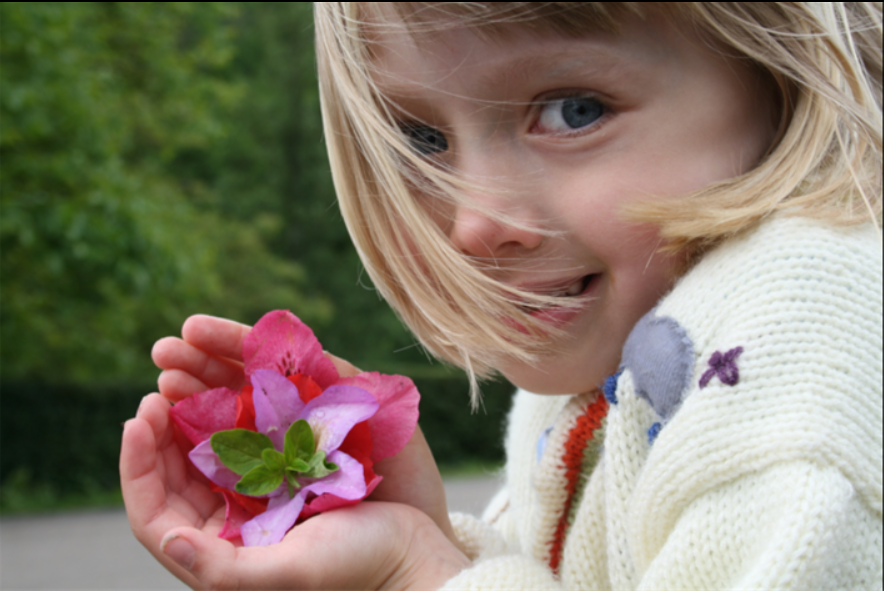
\includegraphics[width=\textwidth]{../images/child.png}
		\caption{Input Image 1}
	\end{subfigure}
	\hfill
	\begin{subfigure}{0.45\textwidth}
		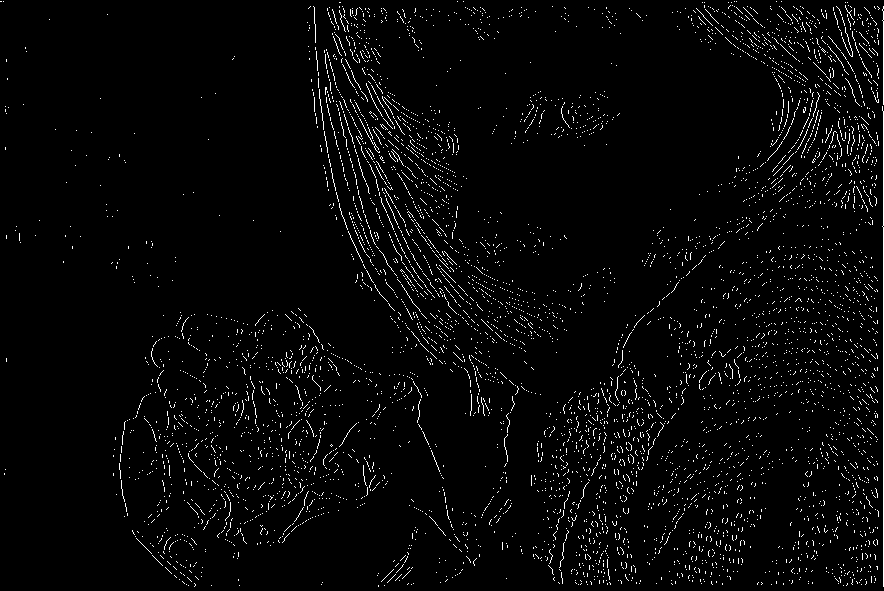
\includegraphics[width=\textwidth]{../results/child.png}
		\caption{Edge Detection Output 1}
	\end{subfigure}

	\vspace{0.5cm}

	\begin{subfigure}{0.45\textwidth}
		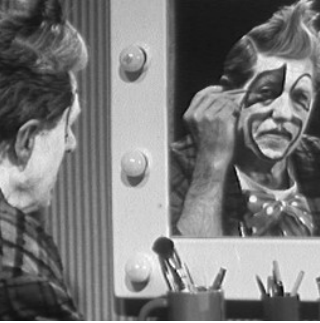
\includegraphics[width=\textwidth]{../images/joker.png}
		\caption{Input Image 2}
	\end{subfigure}
	\hfill
	\begin{subfigure}{0.45\textwidth}
		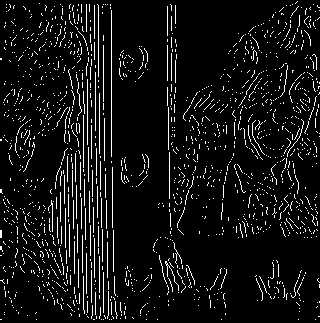
\includegraphics[width=\textwidth]{../results/joker.png}
		\caption{Edge Detection Output 2}
	\end{subfigure}

	\caption{Edge Detection Results for Various Input Images}
\end{figure}

\clearpage

\begin{figure}[!ht]
	\centering

	\begin{subfigure}{0.45\textwidth}
		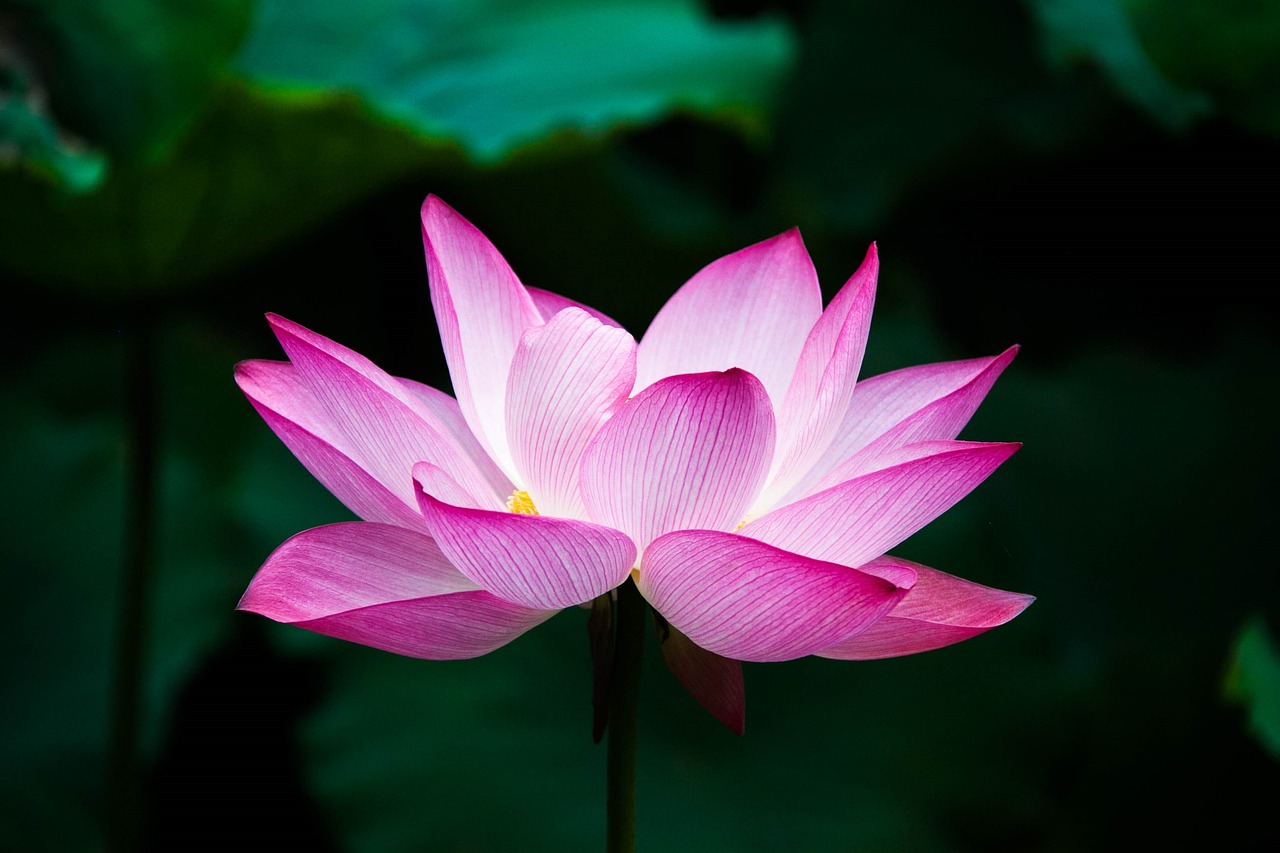
\includegraphics[width=\textwidth]{../images/lotus.jpg}
		\caption{Input Image 3}
	\end{subfigure}
	\hfill
	\begin{subfigure}{0.45\textwidth}
		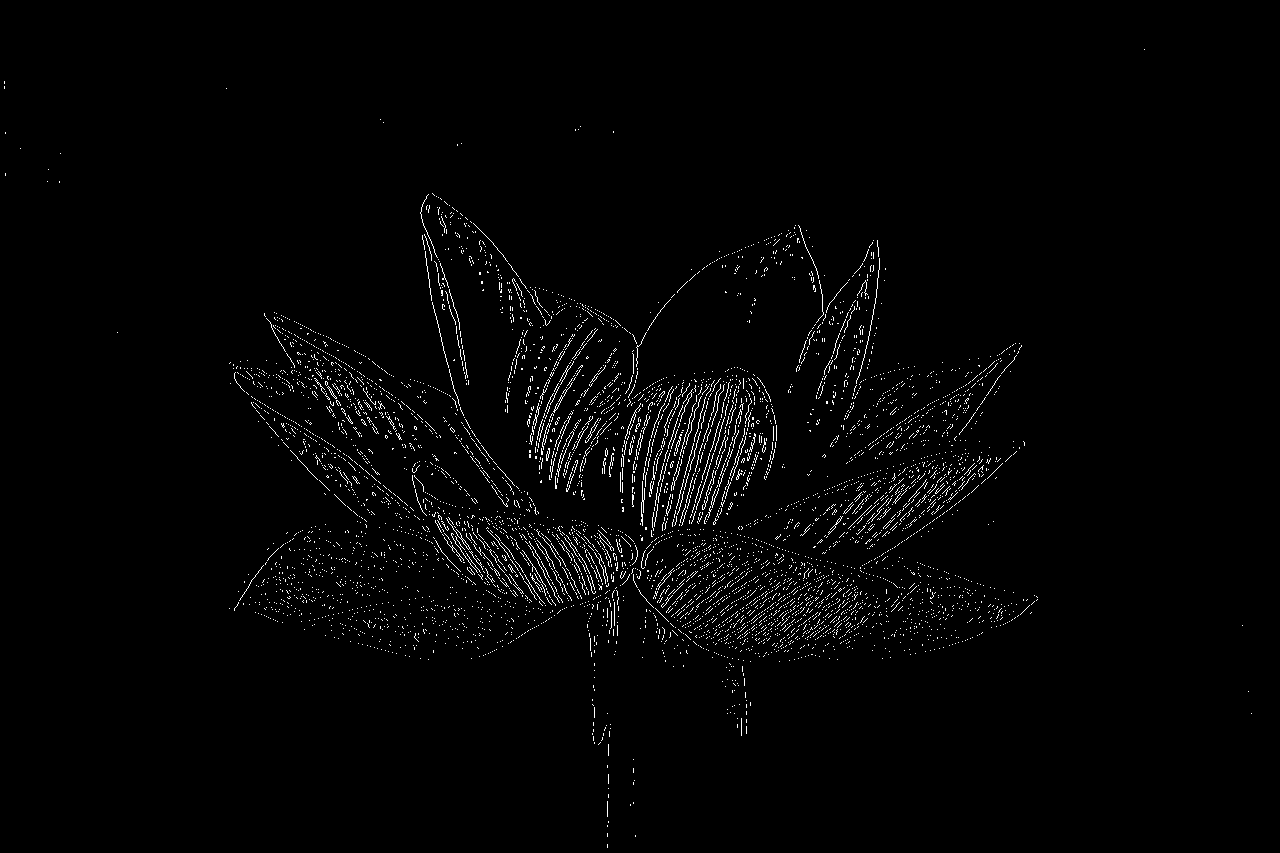
\includegraphics[width=\textwidth]{../results/lotus.png}
		\caption{Edge Detection Output 3}
	\end{subfigure}

	\vspace{0.2cm}

	\begin{subfigure}{0.4\textwidth}
		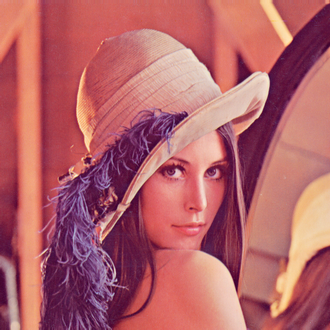
\includegraphics[width=\textwidth]{../images/lenna.png}
		\caption{Input Image 4}
	\end{subfigure}
	\hfill
	\begin{subfigure}{0.4\textwidth}
		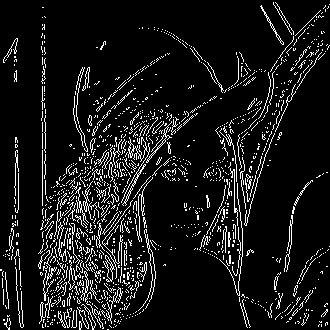
\includegraphics[width=\textwidth]{../results/lenna.png}
		\caption{Edge Detection Output 4}
	\end{subfigure}

	\caption{Edge Detection Results for Various Input Images}
\end{figure}

\section*{Drawbacks}
Some of the drawbacks of using this approach are:

\begin{itemize}
	\item The edges detected are often not continuous and may contain breaks, making it challenging to identify complete object boundaries.
	\item The performance of the method is sensitive to the choice of the \(\sigma\) value in the LoG filter, which can affect the detection of fine details or larger structures.
	\item Thresholding requires careful selection of the threshold value, as inappropriate values can result in missing edges or excessive noise.
	\item The method is computationally intensive due to the convolution with the LoG kernel, especially for large images or high \(\sigma\) values.
\end{itemize}

\section*{Conclusion}
This project demonstrates the use of the Laplacian of Gaussian filter for edge detection, providing flexibility to the user by allowing custom sigma and threshold values.


\end{document}
